% Options for packages loaded elsewhere
% Options for packages loaded elsewhere
\PassOptionsToPackage{unicode}{hyperref}
\PassOptionsToPackage{hyphens}{url}
\PassOptionsToPackage{dvipsnames,svgnames,x11names}{xcolor}
%
\documentclass[
  letterpaper,
  DIV=11,
  numbers=noendperiod,
  oneside]{scrartcl}
\usepackage{xcolor}
\usepackage[left=1in,marginparwidth=2.0666666666667in,textwidth=4.1333333333333in,marginparsep=0.3in]{geometry}
\usepackage{amsmath,amssymb}
\setcounter{secnumdepth}{-\maxdimen} % remove section numbering
\usepackage{iftex}
\ifPDFTeX
  \usepackage[T1]{fontenc}
  \usepackage[utf8]{inputenc}
  \usepackage{textcomp} % provide euro and other symbols
\else % if luatex or xetex
  \usepackage{unicode-math} % this also loads fontspec
  \defaultfontfeatures{Scale=MatchLowercase}
  \defaultfontfeatures[\rmfamily]{Ligatures=TeX,Scale=1}
\fi
\usepackage{lmodern}
\ifPDFTeX\else
  % xetex/luatex font selection
\fi
% Use upquote if available, for straight quotes in verbatim environments
\IfFileExists{upquote.sty}{\usepackage{upquote}}{}
\IfFileExists{microtype.sty}{% use microtype if available
  \usepackage[]{microtype}
  \UseMicrotypeSet[protrusion]{basicmath} % disable protrusion for tt fonts
}{}
\makeatletter
\@ifundefined{KOMAClassName}{% if non-KOMA class
  \IfFileExists{parskip.sty}{%
    \usepackage{parskip}
  }{% else
    \setlength{\parindent}{0pt}
    \setlength{\parskip}{6pt plus 2pt minus 1pt}}
}{% if KOMA class
  \KOMAoptions{parskip=half}}
\makeatother
% Make \paragraph and \subparagraph free-standing
\makeatletter
\ifx\paragraph\undefined\else
  \let\oldparagraph\paragraph
  \renewcommand{\paragraph}{
    \@ifstar
      \xxxParagraphStar
      \xxxParagraphNoStar
  }
  \newcommand{\xxxParagraphStar}[1]{\oldparagraph*{#1}\mbox{}}
  \newcommand{\xxxParagraphNoStar}[1]{\oldparagraph{#1}\mbox{}}
\fi
\ifx\subparagraph\undefined\else
  \let\oldsubparagraph\subparagraph
  \renewcommand{\subparagraph}{
    \@ifstar
      \xxxSubParagraphStar
      \xxxSubParagraphNoStar
  }
  \newcommand{\xxxSubParagraphStar}[1]{\oldsubparagraph*{#1}\mbox{}}
  \newcommand{\xxxSubParagraphNoStar}[1]{\oldsubparagraph{#1}\mbox{}}
\fi
\makeatother


\usepackage{longtable,booktabs,array}
\newcounter{none} % for unnumbered tables
\usepackage{calc} % for calculating minipage widths
% Correct order of tables after \paragraph or \subparagraph
\usepackage{etoolbox}
\makeatletter
\patchcmd\longtable{\par}{\if@noskipsec\mbox{}\fi\par}{}{}
\makeatother
% Allow footnotes in longtable head/foot
\IfFileExists{footnotehyper.sty}{\usepackage{footnotehyper}}{\usepackage{footnote}}
\makesavenoteenv{longtable}
\usepackage{graphicx}
\makeatletter
\newsavebox\pandoc@box
\newcommand*\pandocbounded[1]{% scales image to fit in text height/width
  \sbox\pandoc@box{#1}%
  \Gscale@div\@tempa{\textheight}{\dimexpr\ht\pandoc@box+\dp\pandoc@box\relax}%
  \Gscale@div\@tempb{\linewidth}{\wd\pandoc@box}%
  \ifdim\@tempb\p@<\@tempa\p@\let\@tempa\@tempb\fi% select the smaller of both
  \ifdim\@tempa\p@<\p@\scalebox{\@tempa}{\usebox\pandoc@box}%
  \else\usebox{\pandoc@box}%
  \fi%
}
% Set default figure placement to htbp
\def\fps@figure{htbp}
\makeatother





\setlength{\emergencystretch}{3em} % prevent overfull lines

\providecommand{\tightlist}{%
  \setlength{\itemsep}{0pt}\setlength{\parskip}{0pt}}



 


\KOMAoption{captions}{tableheading}
\makeatletter
\@ifpackageloaded{caption}{}{\usepackage{caption}}
\AtBeginDocument{%
\ifdefined\contentsname
  \renewcommand*\contentsname{Table of contents}
\else
  \newcommand\contentsname{Table of contents}
\fi
\ifdefined\listfigurename
  \renewcommand*\listfigurename{List of Figures}
\else
  \newcommand\listfigurename{List of Figures}
\fi
\ifdefined\listtablename
  \renewcommand*\listtablename{List of Tables}
\else
  \newcommand\listtablename{List of Tables}
\fi
\ifdefined\figurename
  \renewcommand*\figurename{Figure}
\else
  \newcommand\figurename{Figure}
\fi
\ifdefined\tablename
  \renewcommand*\tablename{Table}
\else
  \newcommand\tablename{Table}
\fi
}
\@ifpackageloaded{float}{}{\usepackage{float}}
\floatstyle{ruled}
\@ifundefined{c@chapter}{\newfloat{codelisting}{h}{lop}}{\newfloat{codelisting}{h}{lop}[chapter]}
\floatname{codelisting}{Listing}
\newcommand*\listoflistings{\listof{codelisting}{List of Listings}}
\makeatother
\makeatletter
\makeatother
\makeatletter
\@ifpackageloaded{caption}{}{\usepackage{caption}}
\@ifpackageloaded{subcaption}{}{\usepackage{subcaption}}
\makeatother
\makeatletter
\@ifpackageloaded{sidenotes}{}{\usepackage{sidenotes}}
\@ifpackageloaded{marginnote}{}{\usepackage{marginnote}}
\makeatother
\usepackage{bookmark}
\IfFileExists{xurl.sty}{\usepackage{xurl}}{} % add URL line breaks if available
\urlstyle{same}
% fallback for those not using the hyperref driver hyperxmp:
\makeatletter
\@ifundefined{xmpquote}{\newcommand{\xmpquote}[1]{#1}}{}
\makeatother
\hypersetup{
  pdftitle={6: Structures and Organizations},
  colorlinks=true,
  linkcolor={blue},
  filecolor={Maroon},
  citecolor={Blue},
  urlcolor={Blue},
  pdfcreator={LaTeX via pandoc}}


\title{6: Structures and Organizations}
\author{}
\date{}
\begin{document}
\maketitle


Now that we understand \href{./Ch_4_Meaning.qmd}{meaning} and
\href{./Ch_5_Interaction.qmd}{socialization and interaction}, we can
take the next step of abstraction in our sociological journey. The
central object of sociological analysis is people-in-society, and the
binding agents connecting them are \textbf{social structures}, the
regular patterns of interaction which organize social life.

Social structures come in three main varieties: groups, organizations,
and networks.

\section{From Aggregates and Groups}\label{from-aggregates-and-groups}

The simplest social structures are groups, which emerge from aggregates.
\textbf{Aggregates} are simple collections of people who happen to be
together in a particular place but do not significantly interact or
identify with one another. \textbf{Groups,} meanwhile, \emph{do}
regularly interact, share expectations about each others' behavior, and
share at least some sense of common identity. As these definitions
imply, the two key distinctions of ``group-ness'' are (1) whether there
is ongoing, regular interaction, and (2) whether members have a sense of
collective identity.

\subsection{Kinds of Groups}\label{kinds-of-groups}

There are two main ways to differentiate kinds of groups. The first is
how intensive, emotionally-laden, and face-to-face the group is. We call
groups that express all of these features strongly \textbf{primary
groups}, and all other kinds of groups \textbf{secondary
groups}.\sidenote{\footnotesize There are ambiguous cases that are not clearly primary
  or secondary groups. For instance, what about a very intensive on-line
  e-sports team? Or what about a religious \emph{denomination} versus a
  specific \emph{church} or \emph{congregation}?} One example of this is
sports teams: if you play on a serious team, chances are you are
participating in a \emph{primary} group, since you'll see people often
at practice, interact with them face-to-face, and being a part of that
team probably matters a lot to your self-identity. Meanwhile, if you
\emph{cheer for} a team, you might still think of yourself as a part of
that team's ``fandom,'' but you don't directly interact with everyone
outside of getting together to cheer for your team, and (if you're
healthy), your fan affiliation is a less-salient part of your identity.

At a higher level of generality/abstraction, there is another way to
distinguish kinds of groups. At the most general level, all groups
depend on \textbf{in-group/out-group distinctions}, which is to say,
they depend on their force on the claim that there is \emph{some}
fundamental difference within a population between members of an
\textbf{in-group} and those of an \textbf{out-group}. The in-group is
usually said to have higher status and privilege than the out-group, and
the disitinction between then can be the basis for exclusion or even
violence. Because groups are fundamentally social constructions,
however, it is rarely predictable exactly \emph{what} will form the
basis of categorical in-group/out-group distinctions, and they typically
range across all possible bases for identity.

We also use our membership in groups as a standard to judge the
propriety of our own behaviors. We call these groups \textbf{reference
groups} and they can either be concrete (in the case of asking ``what
would my family think of this decision'') or imagined (in the case of
asking ``I want to be a doctor, and what would doctors think of taking
this class''?)

\subsection{Group Size}\label{group-size}

\subsection{Conformity and Groups}\label{conformity-and-groups}

\section{From Groups to
Organizations}\label{from-groups-to-organizations}

\subsection{Especially Formal, Modern Organizations:
Bureaucracies}\label{especially-formal-modern-organizations-bureaucracies}

From antiquity, there has been a case of formal organization that has
played a special historical role, and, in the modern era, has become
\emph{the} mode of organizing complex social life: the
\textbf{bureaucracy}. This kind of organization is distinguished from
others by its very high degree of \textbf{formal rationalization}, which
is to say, the extent to which its features efficiently and effectively
deliver any given end.

The sociologist Max Weber outlined seven features of what he called the
``ideal type'' of bureaucracy:\sidenote{\footnotesize Here, we can treat an ideal type
  as similar to an index: a bureaucracy is ``more of'' a bureaucracy the
  more of these features it fulfills; but not every bureaucracy has
  every single one of these features to the same degree. However, the
  most extreme bureaucracy we can imagine would have them all and
  express them intensively.}

\begin{enumerate}
\def\labelenumi{\arabic{enumi}.}
\tightlist
\item
  \emph{Defined Jurisdictional Areas.} Bureaucratic organizational
  positions are defined by the ``domains'' they oversee. At Stony Brook,
  for instance, I am a professor \emph{of sociology,} and therefore
  cannot automatically teach courses in other disciplines, because they
  are ``not in my area.''
\item
  \emph{Expert Training.} Bureaucratic positions are defined by their
  holders' \emph{expertise}, which is to say demonstrated qualification
  for the position. In complex societies, moreover, it is usually
  impossible to verify training through personal networks and direct
  experience of a person alone, so organizations usually supplement such
  measures with credentials, such as, in the case of university
  professors, the highest academic degrees in their disciplines (usually
  a PhD).
\item
  \emph{Clear-Cut Hierarchy.} In an ideal-typical bureaucracy, defined
  jurisdictional areas carry hierarchies with them; just as people have
  areas they oversee, so too do their underlings have clear lines of
  authority that trace their way up to the overall leader of the
  organization. This means that, when this go wrong, there are clear
  avenues of responsibility and appeal from one person to their
  supervisor, all the way up to the head of the organization.
\item
  \emph{Written Rules of Conduct and Procedure.} Bureaucracies rely on
  cultural technologies to function, and one of the most important is
  writing. On the one hand, written records themselves enable the
  processing of vast inputs and outputs (whether people, goods, or even
  knowledge) through a bureaucracy, not least because writing allows
  each of those inputs and outputs to be abstractly represented, and
  consequently structurally-equivalent officials can deal with the same
  ``case'' based on that case's ``file,'' without needing personal
  knowledge of the history of that case. On the other hand,
  bureaucracies often have extremely intricate written procedures for
  how officials themselves should go about their work, which means that,
  when they deviate from these prescribed norms of behavior, they can be
  held accountable.
\item
  \emph{Full-time Salaried Officials.} Bureaucrats are so effective, in
  part, because they can concentrate on their jobs. This sounds simple,
  but think about how hard it would be for someone to master the
  ins-and-outs of working with bureaucratic cases if they \emph{also}
  had to worry about another position, and consequently could only be
  around for restricted hours, devote comparatively little time to the
  organization, and so on.
\item
  \emph{Separation between Organizational and Private Life.}
  Bureaucracies are at their most efficient when an individual
  bureaucrat is ``separable'' from their job. That is, in principle
  \emph{any} qualified and trained candidate could do the same work as
  any individual bureaucrat, and so the organization does not depend on
  the particular characteristics of any one worker.
\item
  \emph{Organizational Ownership fo the Means of Production.} Finally,
  bureaucracies work so efficiently, in part, because they do not depend
  on any individual bureaucrat's possessions to function, and instead
  the organizations supply their own. Think, again, of Stony Brook: if
  they asked every member of physical plant (the organizational division
  that does maintenance on buildings and grounds) to use their own
  trucks at work, that would only work if (a) everyone had trucks of
  their own to use, and (b) individually was willing to use them for
  work. It is \emph{far} more efficient for Stony Brook to maintain a
  fleet of its own vehicles and equipment to make sure that its
  facilities are actually maintained.
\end{enumerate}

The hallmark of bureaucracy, as shown below, is the organizational
chart. (This one is from the Stony Brook College of Business, but you
could replicate it for literally any bureaucracy you want; they're very
common.) Note how it expresses clear organizational hierarchy (points 1
and 3 above), and carefully delimits the expertise different positions
at different ranks hold (point 2; a ``Professor of Practice,'' for
instance, need not have a PhD, whereas an Assistant, Associate, or Full
Professor does). And the very document itself is a written record of the
conduct and procedures fo the unit, insofar as it can be referred to if
someone is ``out of their lane'' (point 4).

\begin{figure}[H]

{\centering \pandocbounded{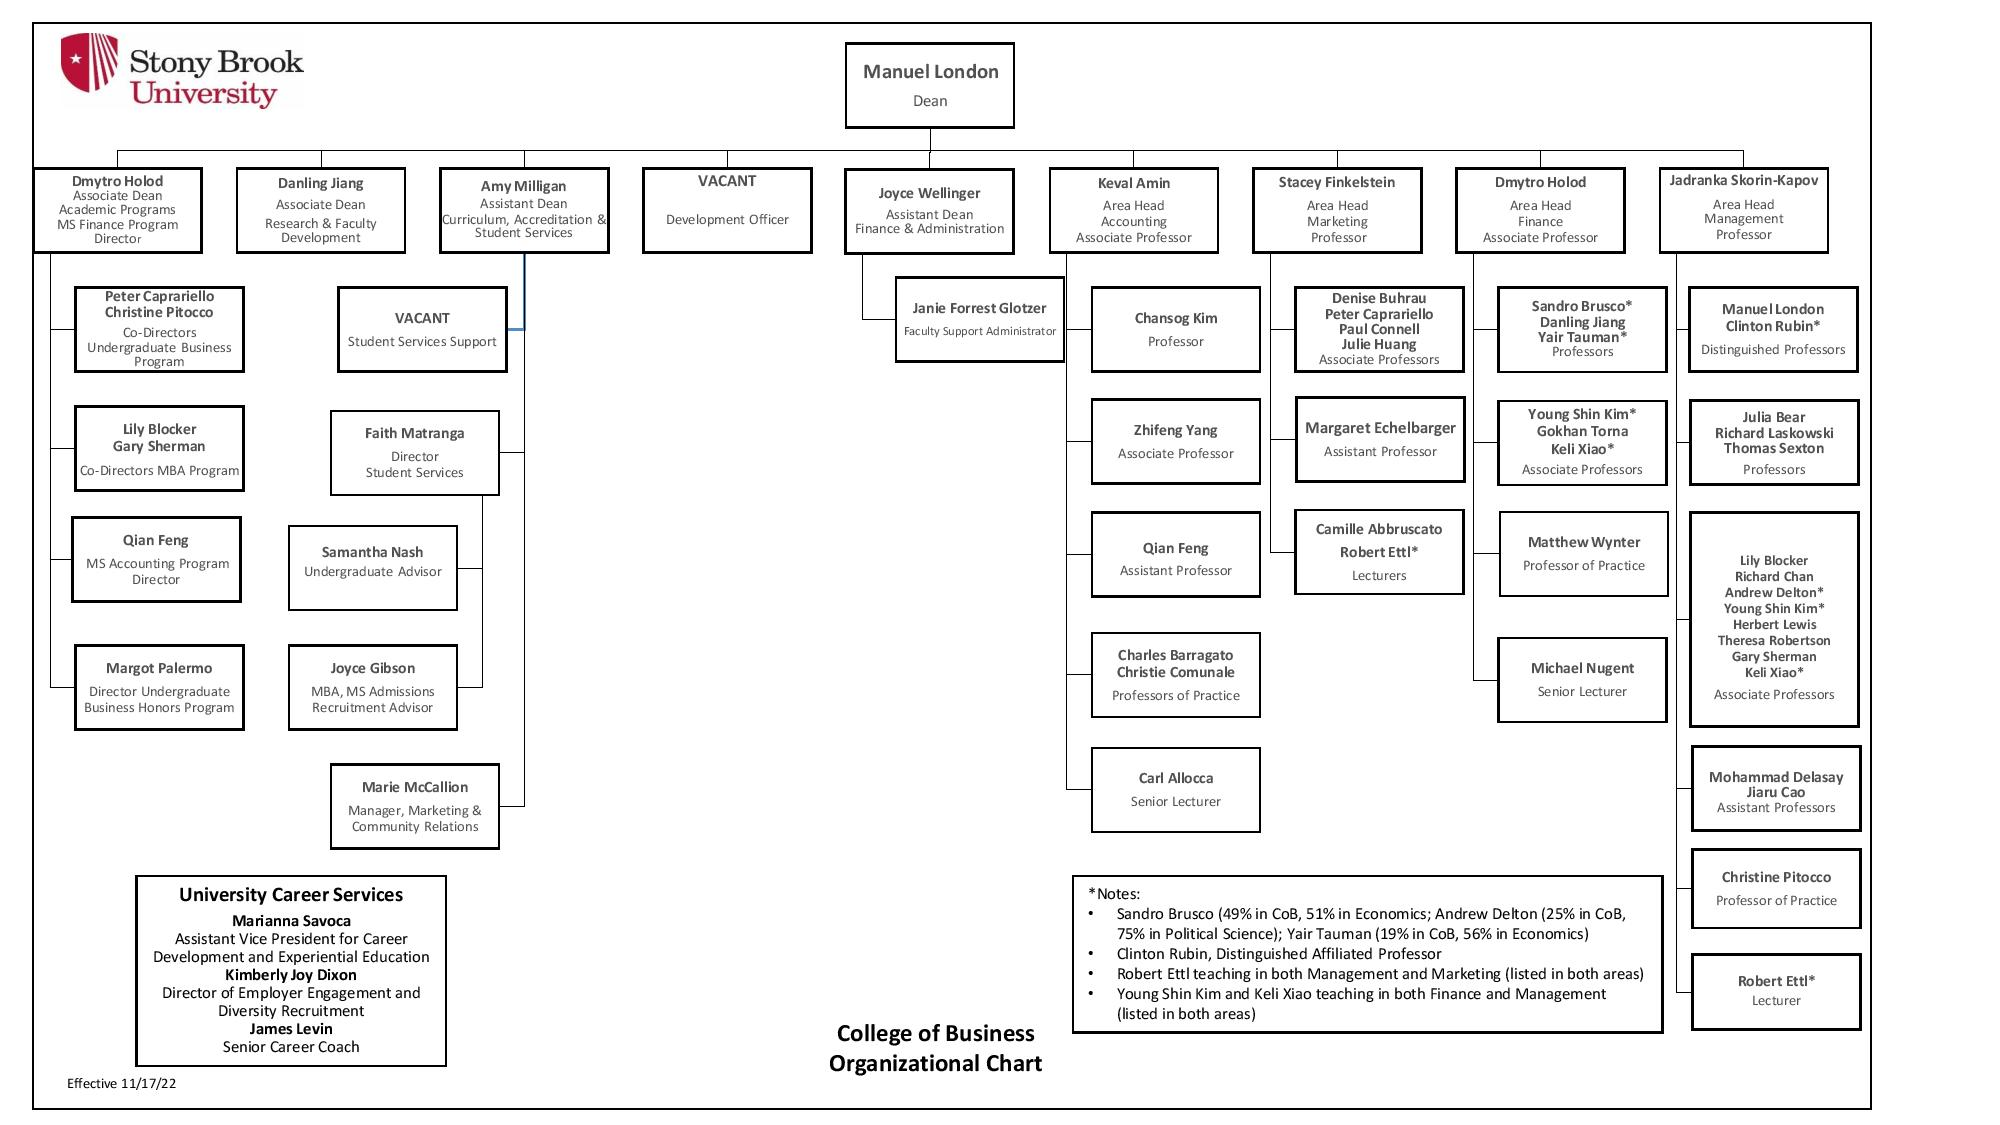
\includegraphics[keepaspectratio]{../images/6_org_chart.png}}

}

\caption{Organization Chart, Stony Brook College of Business}

\end{figure}%

\subsection{The Functions and Dysfunctions of Formal
Organizations}\label{the-functions-and-dysfunctions-of-formal-organizations}

\subsubsection{Functions}\label{functions}

In mainstream American culture, we are used to thinking of bureaucracies
as ineffecient and ``bad.'' But I want to argue that the story is more
complicated. To begin with, consider ``the government,'' in all its
messiness. We're used to thinking of the government as a source of
red-tape and impediments, but if you consider its size relative to the
rest of the United States, you quickly get a sense of how few people are
able to undertake all the functions that keep society functioning. To
begin with, we can see that the federal government is made up of about 3
million people (here excluding the military).

\begin{figure}[H]

{\centering \pandocbounded{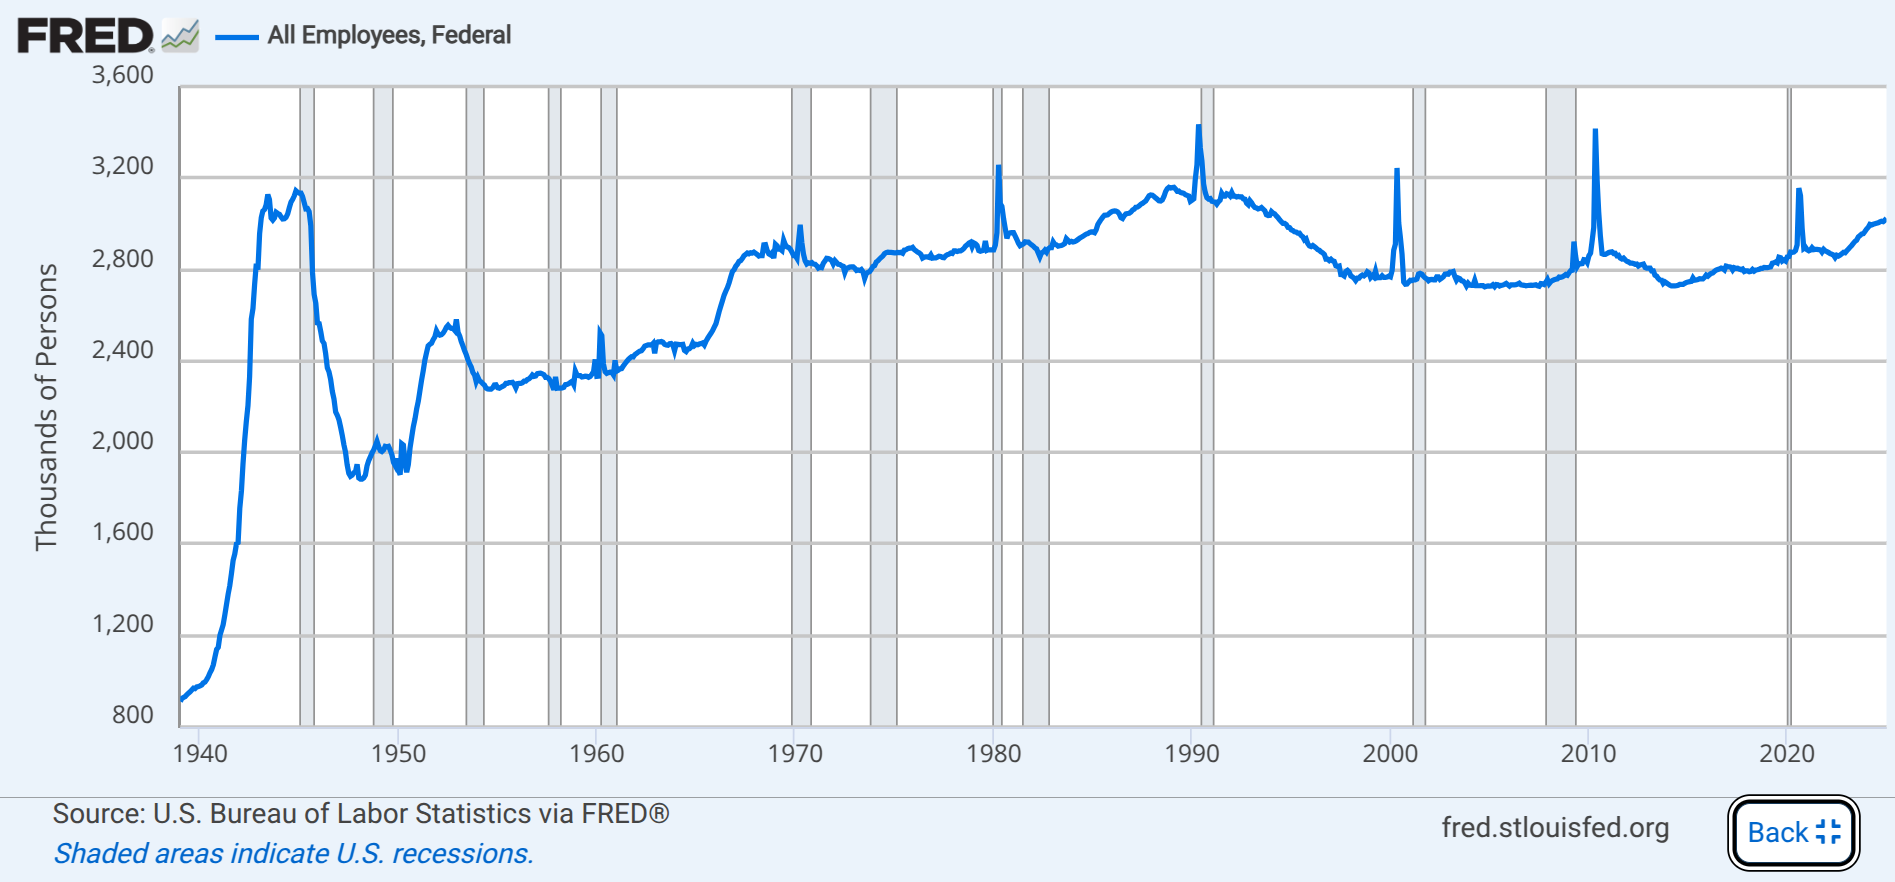
\includegraphics[keepaspectratio]{../images/6_fed_size.png}}

}

\caption{The Rough Size of the Federal Government}

\end{figure}%

And we can add state, county, and local government employees to that
count as well (which would, by the way, include SUNY professors like
me---we are state employees!), which would boost that count to just shy
of 24 million people.

\begin{figure}[H]

{\centering \pandocbounded{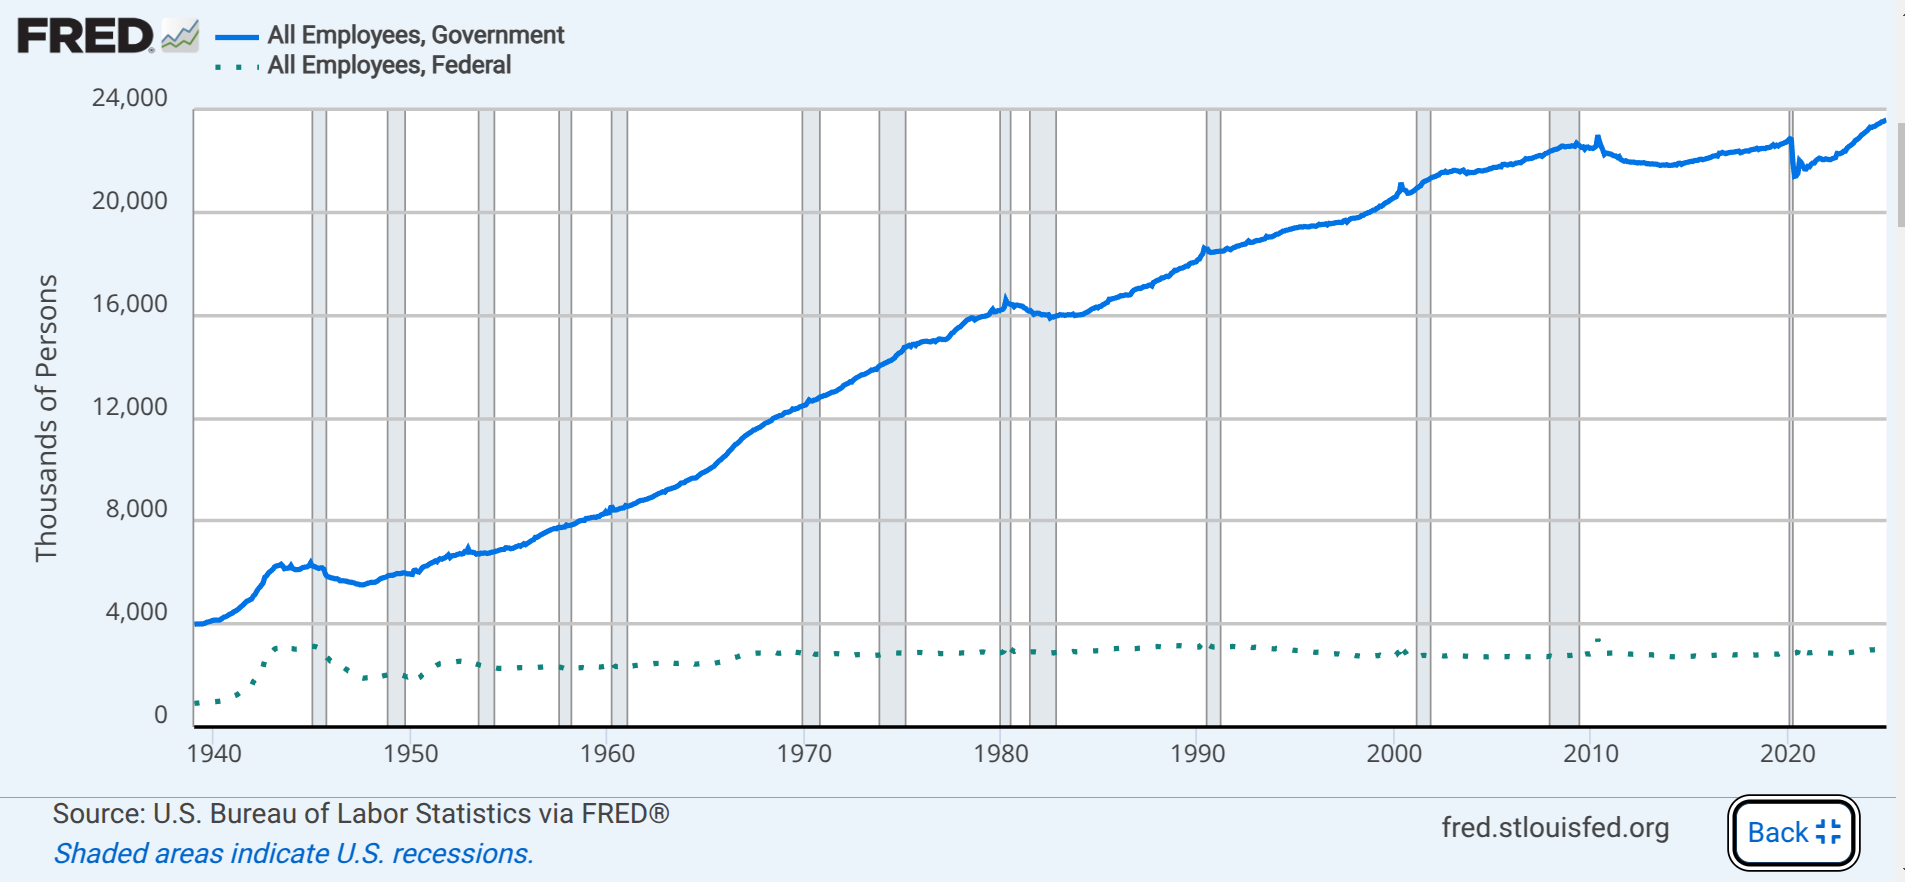
\includegraphics[keepaspectratio]{../images/6_fed_state_size.png}}

}

\caption{The Rough Size of the Federal Government and State Governments}

\end{figure}%

But \emph{then}, if we take a step back, and consider those 27-or-so
million government workers relative to the population of the United
States, we get a sense of how \emph{small} the ``government
bureaucracy'' really is. (The US Census Bureau
\href{https://www.census.gov/popclock/}{estimates} that the US
Population is about 343 million right now, which means that Government
at all levels adds up to just under 8\% of the total population.)

\begin{figure}[H]

{\centering \pandocbounded{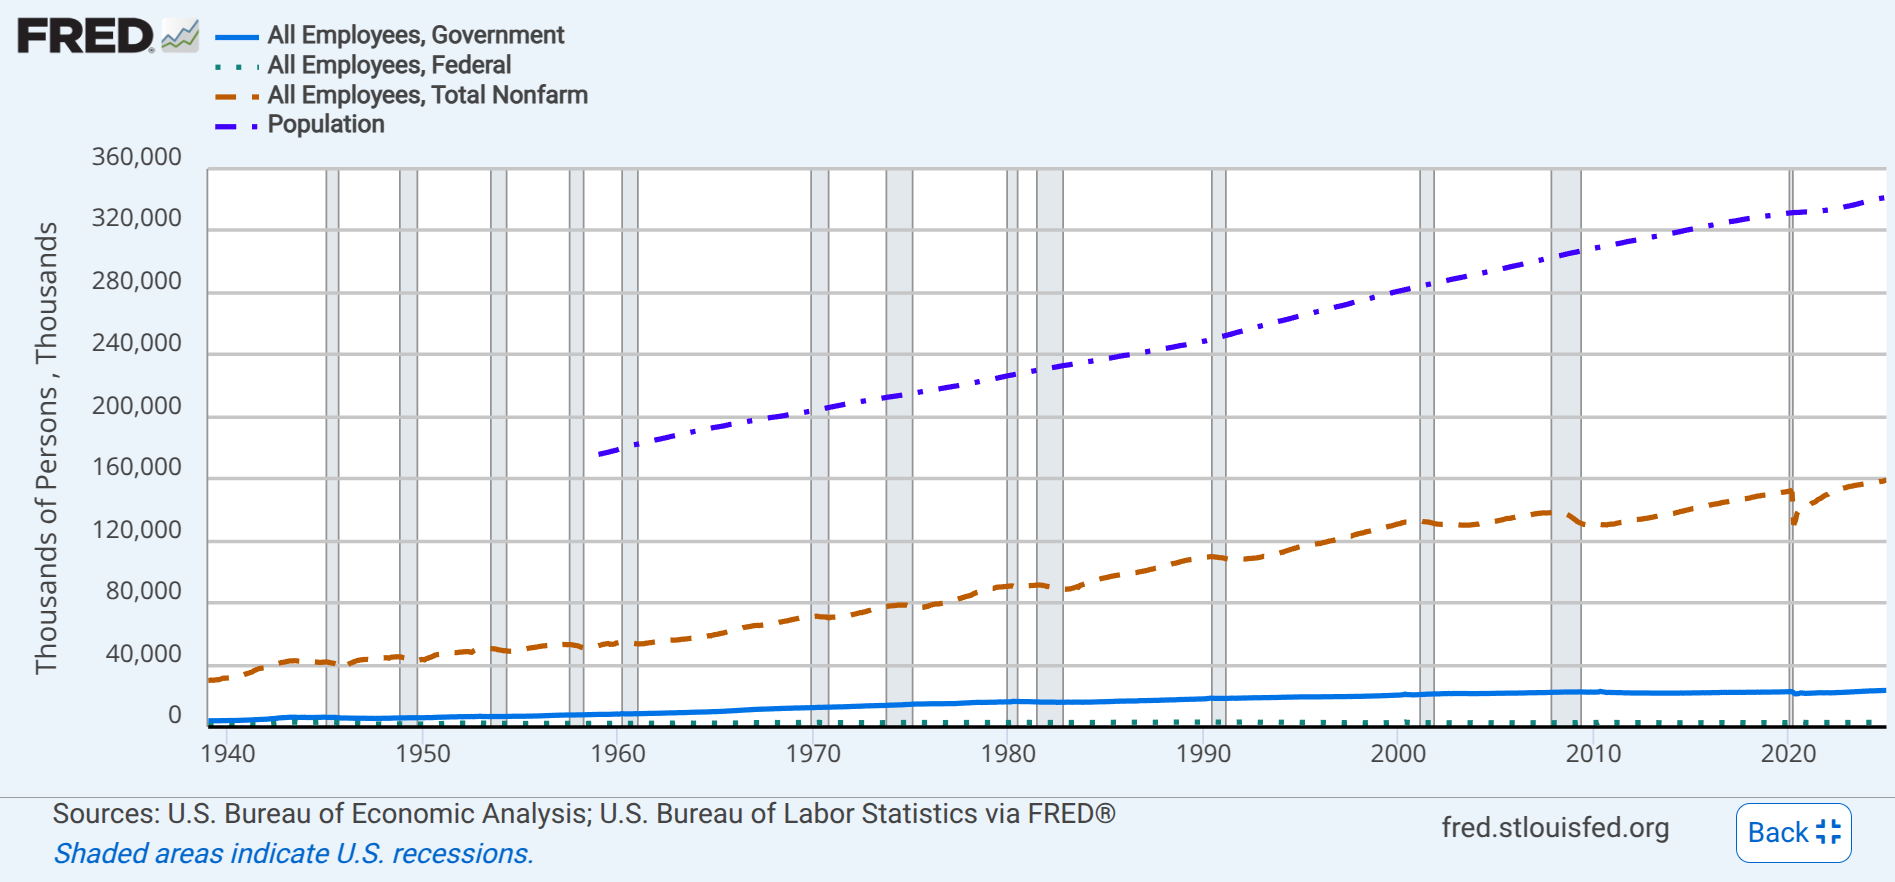
\includegraphics[keepaspectratio]{../images/6_fed_state_size_population.png}}

}

\caption{The Rough Size of the Government, Compared to Population}

\end{figure}%

\subsubsection{Dysfunctions}\label{dysfunctions}

At the same time that bureaucracies are impressively effective, they
also manifest negative functions. One of the biggest comes from a point
implied by bureaucracy's very efficiency: as organizations,
bureaucracies can very efficiency pursue \emph{given} ends, but it can
sometimes be difficult to get them to stick to the ends that they have
been given. That is an elliptical way of saying that bureaucracies can
sometimes become \textbf{decoupled} from their designed purposes,
beginning to pursue different ends. When we accuse an organization of
``losing its way,'' for instance, what we typically mean that it was
designed for an explicit purpose, but has drifted to actually pursuing
another.

Another ``dysfunction'' (which you might actually view as a
``function,'' depending on your value commitments) of bureaucracies is
that when they inputs and outputs of bureaucracy are \emph{people}, the
very value-neutrality and efficiency of bureaucratic operations mean
that discipline, control, and even violence can be exerted by a small
minority on very large populations. The historian and social theorist
Michel Foucault called this effective discipline \textbf{panopticism},
which he built from an analogy of the architecture of some prisons.

\begin{figure}[H]

{\centering \pandocbounded{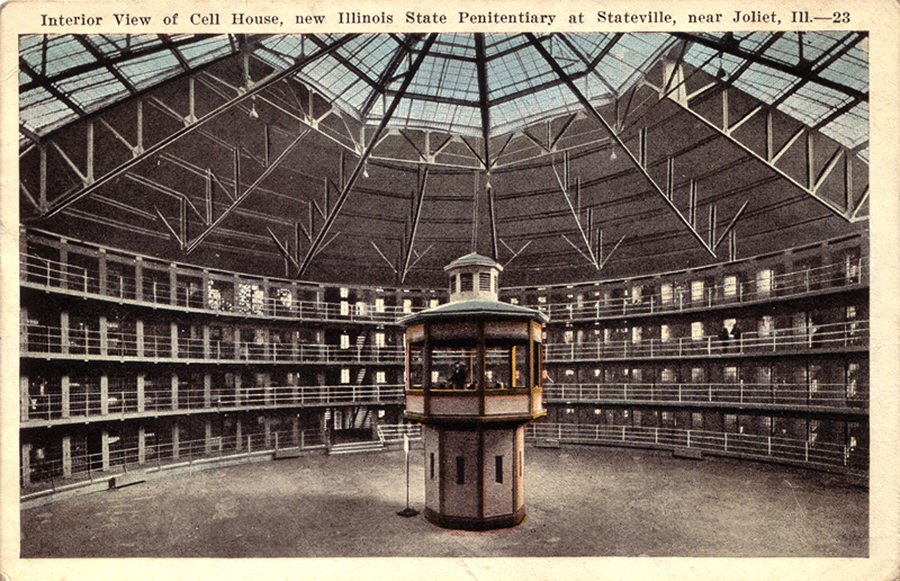
\includegraphics[keepaspectratio]{../images/6_stateville.jpg}}

}

\caption{Stateville Prison, Joliet IL.}

\end{figure}%

Foucault noticed that, given this prison design, all of the prisoners
had to behave \emph{as though} they were under observation at all times.
(Their prison cells were open to the central guard-tower, but they could
not tell if the guard was directly looking into their cells.)
Accordingly, instead of one guard being needed to observe one prisoner,
very few guards could exert discipline on a very large population of
prisoners because of the prison's design.

Foucault thought that panopticism also worked by analogy to describe
formal organizations' power to discipline people, especially when
enabled by technology. Indeed, contemporary examples of panoptic
orgnaizations abound, from consumer-oriented ``nudges'' by apps like
\href{https://www.weightwatchers.com/us/blog/introducing-new-weight-watchers}{diet
monitors},
\href{https://www.reddit.com/r/duolingo/comments/1c2gkt6/sad_duolingo_icon_mega_thread/}{language-learning
programs}, and even
\href{https://www.covenanteyes.com/about/?gad_source=1&gad_campaignid=407188357&gclid=CjwKCAjwxeHWBhBPEiwAiqtQ-aMtPL_Vfnj_ODa3GomXjKMG3YhIVtROQqqOkd4YNbcvgFrxEH8bThoCoKkQAvD_BwE}{anti-pornography
habit-builders} (which all monitor our activity, collect it, and either
digest it back to us or share it with others), to state-sponsored
\href{https://www.flocksafety.com/products/license-plate-readers}{observation
of our movements}, to
\href{https://it.stonybrook.edu/services/respondus}{direct monitoring of
our behavior in the university} through ``virtual proctoring.''

\section{Networks}\label{networks}

\subsection{Findings of Network
Analysis}\label{findings-of-network-analysis}

\subsection{The Interface of Network and
Organization}\label{the-interface-of-network-and-organization}

\section{The Internet and
Organizations}\label{the-internet-and-organizations}




\end{document}
